\documentclass[11pt]{article}
\usepackage{fullpage}
\usepackage{amsmath, amssymb, graphicx, caption}
\graphicspath{{EPS/}}

\title{Errata for \\
      \textbf{Fundamentals of Fiber Orientation} \\
      { \normalsize \texttt{http://github.com/charlestucker3/Fundamentals-of-Fiber-Orientation-errata}} }

\author{Charles L.~Tucker III \\
       Department of Mechanical Science and Engineering \\
        University of Illinois at Urbana-Champaign \\
        1206 W.~Green St. \\
        Urbana, IL 61801 \\
        }
\include{defs}  % Macro definitions

\begin{document}
\maketitle

If you find additional errors, please send them to \texttt{ctucker@illinois.edu} so that they can be included here.

\section*{Chapt.\ 4. Flow Orientation of Single Fibers}

On page 92, the last paragraph, the second line, $\xi > 1$ should be $\xi > 0$.  The corrected sentence should read:
\begin{quote}
If the particle is fiber-shaped ($a > b$) then $\xi > 0$ and this term pulls the fiber toward the direction of maximum stretching rate.
\end{quote}
Thanks to Florian Mallmann for this correction.

\section*{Chapt.\ 4. Flow Orientation of Groups of Fibers}

On page 163, Eqn.~(5.99), the first plus sign on the right-hand side should be a minus sign.  The corrected equation should read
\begin{equation*}
    \dot{\A}^\text{RSC} = \dot{\A} - (1 - \kappa) \sum_{\lambda = 1}^3 \dot{\lambda}_i \ev_i \ev_i
\end{equation*}
Thanks to Julien F\'erec for this correction.

\section*{Chapt.\ 8. Mechanical Properties and Orientation}

The example on page 246 of modeling stiffness vs.~fiber orientation is described as being for a 40\% by weight long glass fiber/PP composite, but the calculations for Fig.~8.5 actually used 30\% by weight.  40\% should be changed to 30\% in the fiber caption and in the second line of the first paragraph on page 246.  Thanks to Huidi Ji for this correction.

The example calculation in Section~8.4.5 for the stiffness of a layered structure states that the long glass fiber/PP composite has 40\% by weight of fibers.  However, the calculations in Fig.~8.6(c) and Table~8.4 actually used 30\% by weight.  The correct figure should look like this:
\begin{figure*}[h]
   \centering
    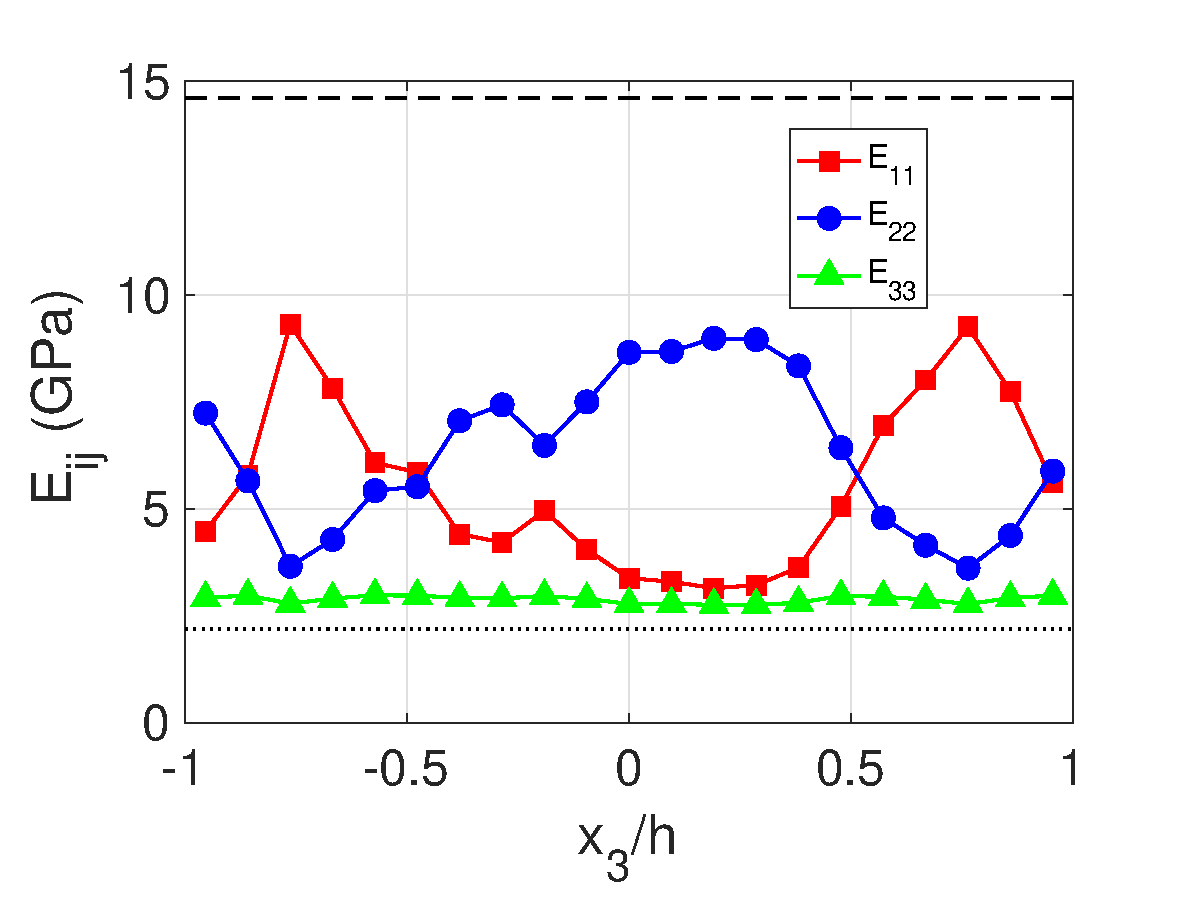
\includegraphics[width = 0.48\textwidth, trim = 0  0 0 0, clip = true, keepaspectratio = true]{FODexample2E.eps} \\
    \caption*{Fig. 8.6(c) Stiffness, 40 wt.\% long glass fiber/PP}
\end{figure*}

\newpage %%%%%%%%%%%%%% REMOVE THIS IN THE NEXT UPDATE %%%%%%%%%%
\noindent The correct table should read:
\begin{table}[h]
    \centering
     \caption*{Table 8.4 Predicted tensile and flexural moduli for the two injection molded samples in Fig. 8.6.}
         \begin{tabular}{l|c|c}
                  & $E_{11}$ (GPa)     & $E_{22}$ (GPa)   \\ 
                  \hline
                  30 wt.\% short glass fiber/PC & & \\
                  ~~~~~~~~ Tensile   & 8.04  & 4.02 \\
                  ~~~~~~~~ Flexural  & 8.51 & 3.75 \\
                  \hline
                  40 wt.\% long glass fiber/PP & & \\
                  ~~~~~~~~ Tensile   & 5.59  & 6.38 \\
                  ~~~~~~~~ Flexural  & 6.58 & 5.42 
           \end{tabular}
    \end{table}
    
\section*{References}

On page 315, reference [KKCO20] has no page number.  The page number should be 69, and the corrected reference should read:
\begin{quote}
\begin{itemize}
\item[{[KKCO20]}] S. K. Kugler, A. Kech, C. Cruz, and T. Osswald. Fiber orientation predictions—A review of existing models. \textit{J. Compos. Sci.}, 4(2):69, 2020.
\end{itemize}
\end{quote}



\end{document}